% !TeX root = ../main.tex
% Add the above to each chapter to make compiling the PDF easier in some editors.

\chapter{Farm Power Model}\label{chapter:power_model}

With the goal of training a model tailor made to the requirements of the optimization problem, the data used for training the model has to generated using a open source simulation method, allowing to set the parameter space of the model as required to the given optimization problem. After investigating the two python based wind farm simulation tools FLORIS and PyWake, FLORIS was chosen due to solid documentation, what appears to be very stable releases and broad functionalities regarding wake modelling. FLORIS is a wind farm simulation tool developed by the National Renewable Energy Laboratory (NREL).



Wind turbine power curve modelling under wake conditions using measurements from a spinner-mounted lidar:
https://www.sciencedirect.com/science/article/pii/S0306261924003684

Floris:
https://github.com/nrel/floris



Main Effects of Wake Turbolence: 
- Wind Speed (needs time to mix with outside airflow)
- Turbolence
\section{Data Source}

\section{Modelling}

To model the relationship between the attributes of a incoming airflow to a wind turbine and the output generated by the same wind turbine many surrogate models could be chosen. As the model generated in this for this thesis is created with the goal of introducing it into the pyomo extension referenced in Chapter \ref{chapter:introduction}, the model has to be compatible with said extension. That is why the model chosen is a simple neural network with limited number of hidden layers and nodes, with the size of the Neural Network being limited for said extension. 

\subsection{Neural Networks and Training of  Neural Networks}

In the following section, a biref introduction is given into how Neural Networks work and are trained.  Fundemanetally, Neural Networks represents Graph Networks consisting out of Function blocks as the nodes, in the case of Neural Networks called perceptron (or Neurons as more general terms) and arcs which correspond to the inputs/outputs of a given perceptron. In simple words, the inputs to the Neurons are summed up and introduced as argument into a function $f()$ which yields a output $y$, representing the output of the given perceptron. These Neurons are organized in layers, which correspond to the row type structure Neural Networks are usually represented in and each perceptron of one layer is connected to every other perceptron of the following layer. The following layer in this case means in the direction of flow, in visualizations usually from left to right. The arcs thus in simple terms correspond to a single number and the Neurons to the action of summing up all inputs and then applying the unspecified function $f()$ to generate a output. This process is repeated for all Neurons in the network, with the first layer of the network taking as input the values of the values of the given data features (the input values to the model) and the last layer producing outputs corresponding to the output value(s) of the model. The number of Neurons in this first and last layer correspond to the task the Neural Network is supposed to perform. If the goal is to identify handwritten numbers 1-9 from 50x50 pixel images, the imput layer might have 50x50 Neurons for the value of each pixel, and the output layer 9 layers with the output value of each perceptron representing how much the networks thinks the given image shows the corresponding numbers 1-9. A schematic of this architecture is given in Figure \ref{fig:neural_network_architecture}.

\begin{figure}[h] 
\centering
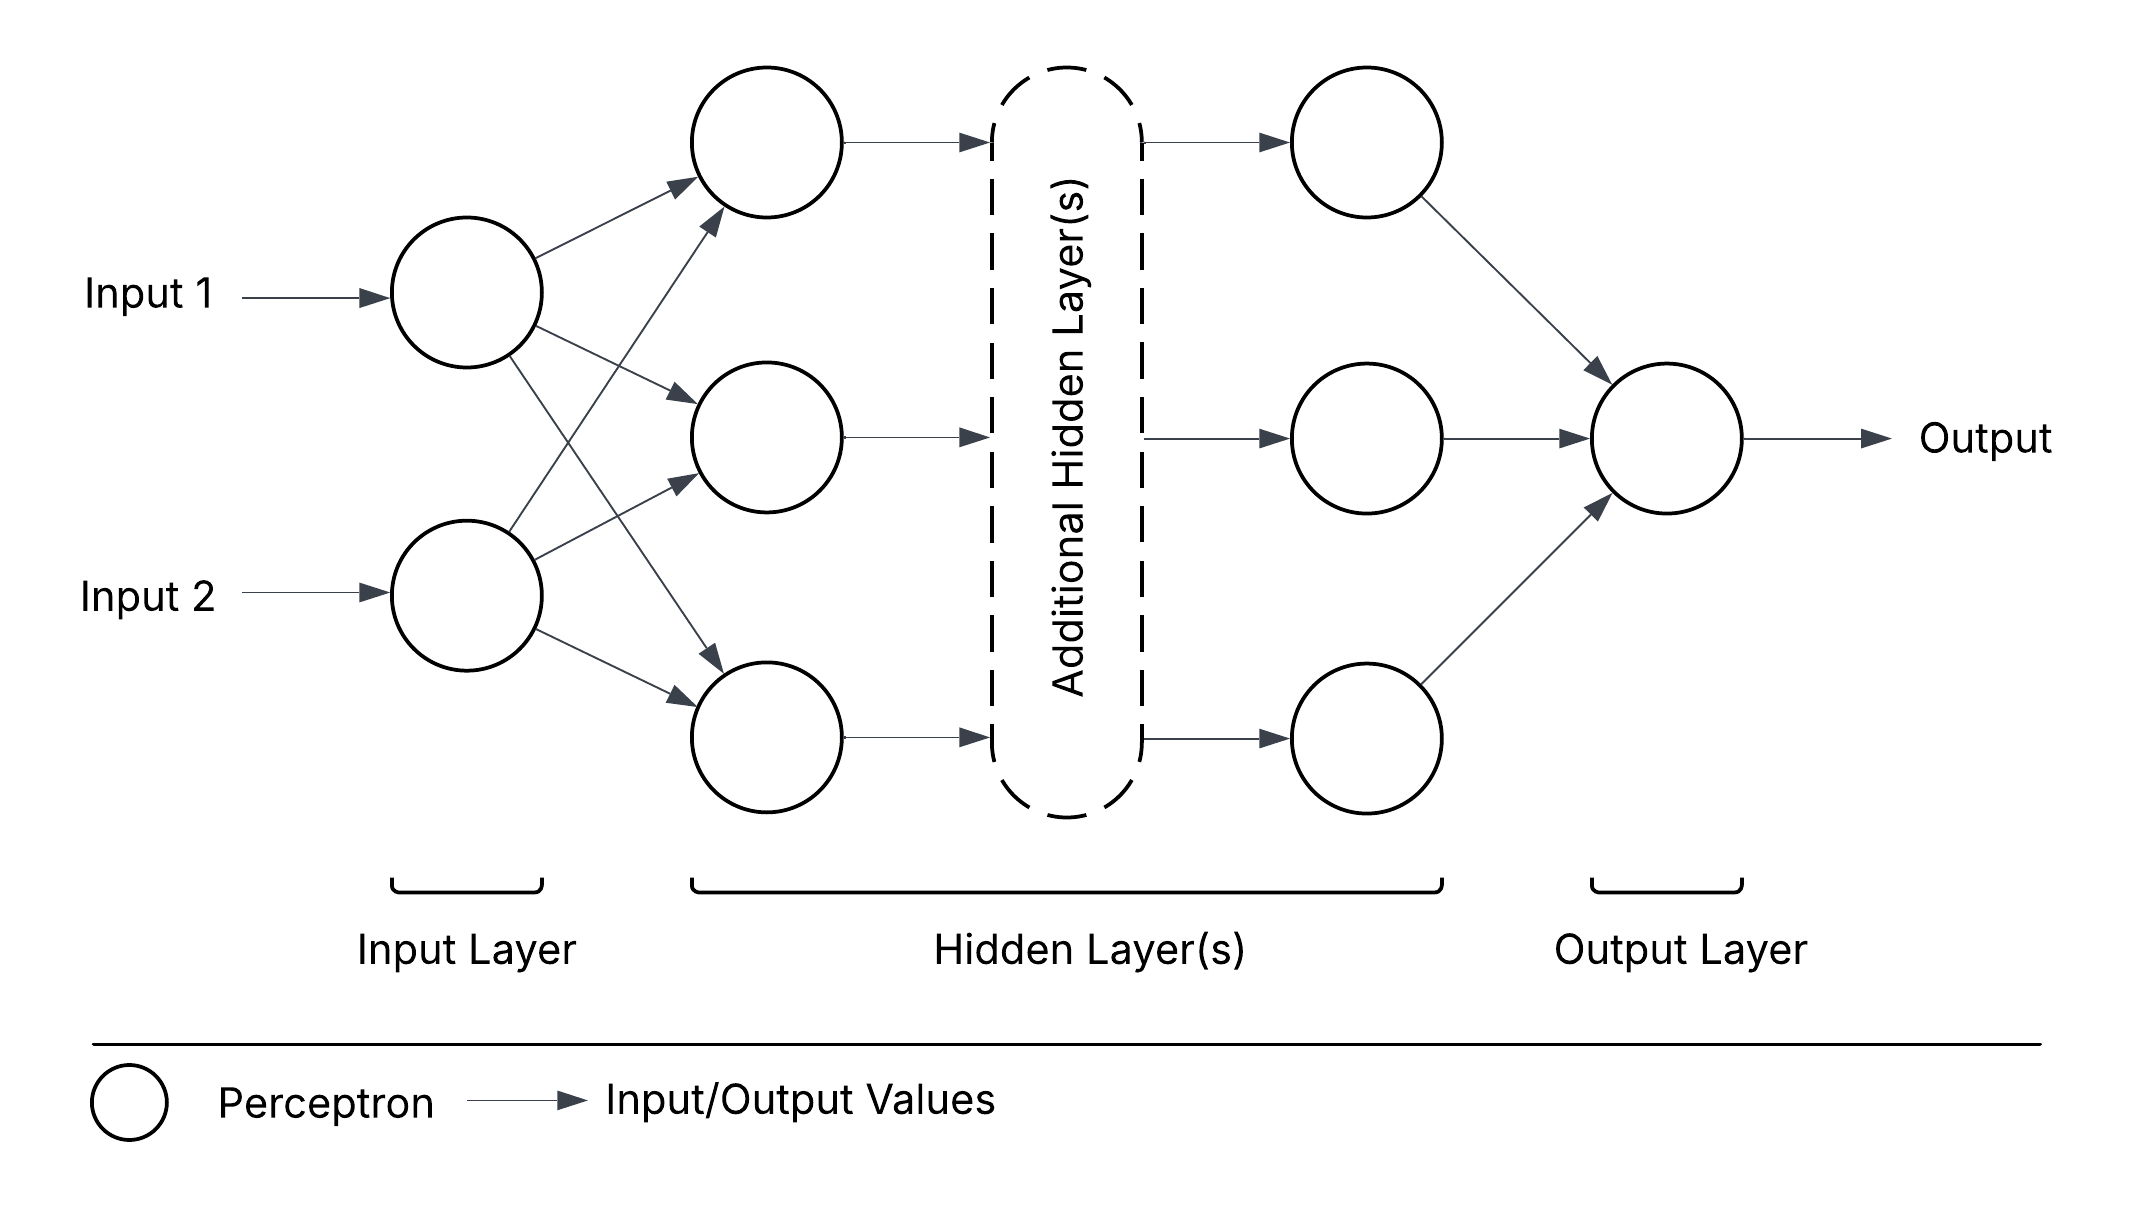
\includegraphics[width=0.9\textwidth]{figures/modelling/neural_network_concept.png} % file name without extension
\caption{Schematic of Neural Network Architecture}
\label{fig:neural_network_architecture}
\end{figure}

As shown in Figure \ref{fig:neuron_calculations} the output of a Neuron is slighlty more complicated as described befoe, as the output $y$ is generated by summing up the inputs $x$ multiplied by a corresponding weight $w$ together with a bias $b$ and introducing this summation as argument into a activation function $f()$. In this process, the weights $w$ represent a weigh to give importance to the individual inputs and the bias $b$ serves to set a minimum output value that will always be reached, regardless of the inputs. 

\begin{figure}[h] 
	\centering
	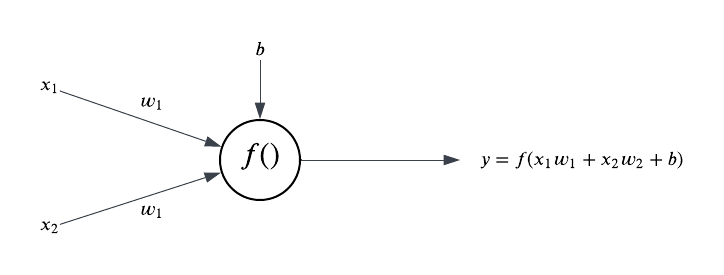
\includegraphics[width=0.8\textwidth]{figures/modelling/perceptron_concept.png} % file name without extension
	\caption{The output of a neuron is generated by applying the activation function to the sum as the weighted inputs $w_ix_i$ and the bias of the neuron $b$}
	\label{fig:neuron_calculations}
\end{figure}

The activation function $f()$ is called activation function, as in its most simplest form it represents a step function that decides if a neuron activates or not, e.g. takes the binary values ${0,1}$ for a given threshhold. Contrary to the human brain where neurons are indeed binary, most Neural Networks resort to a activation function whose outputs are not binary but deliver continious values between $0$ and $1$ to avoid the boundary issues that occour with binary threshholds. The most common function used instead of a step function is the sigmoid function, which roughly corresponds to a continuous version of the step function, with $\sigma(x) \approx 1$ for $x \to \infty$ and $\sigma(x) \approx 0$ for $x \to -\infty$.


\[
\sigma(x) = \frac{1}{1 + e^{-x}}
\]

This relationship also becomes aparent when plotting both of those functions over each other, as shown in \ref{fig:activation_functions}

\begin{figure}[h] 
	\centering
	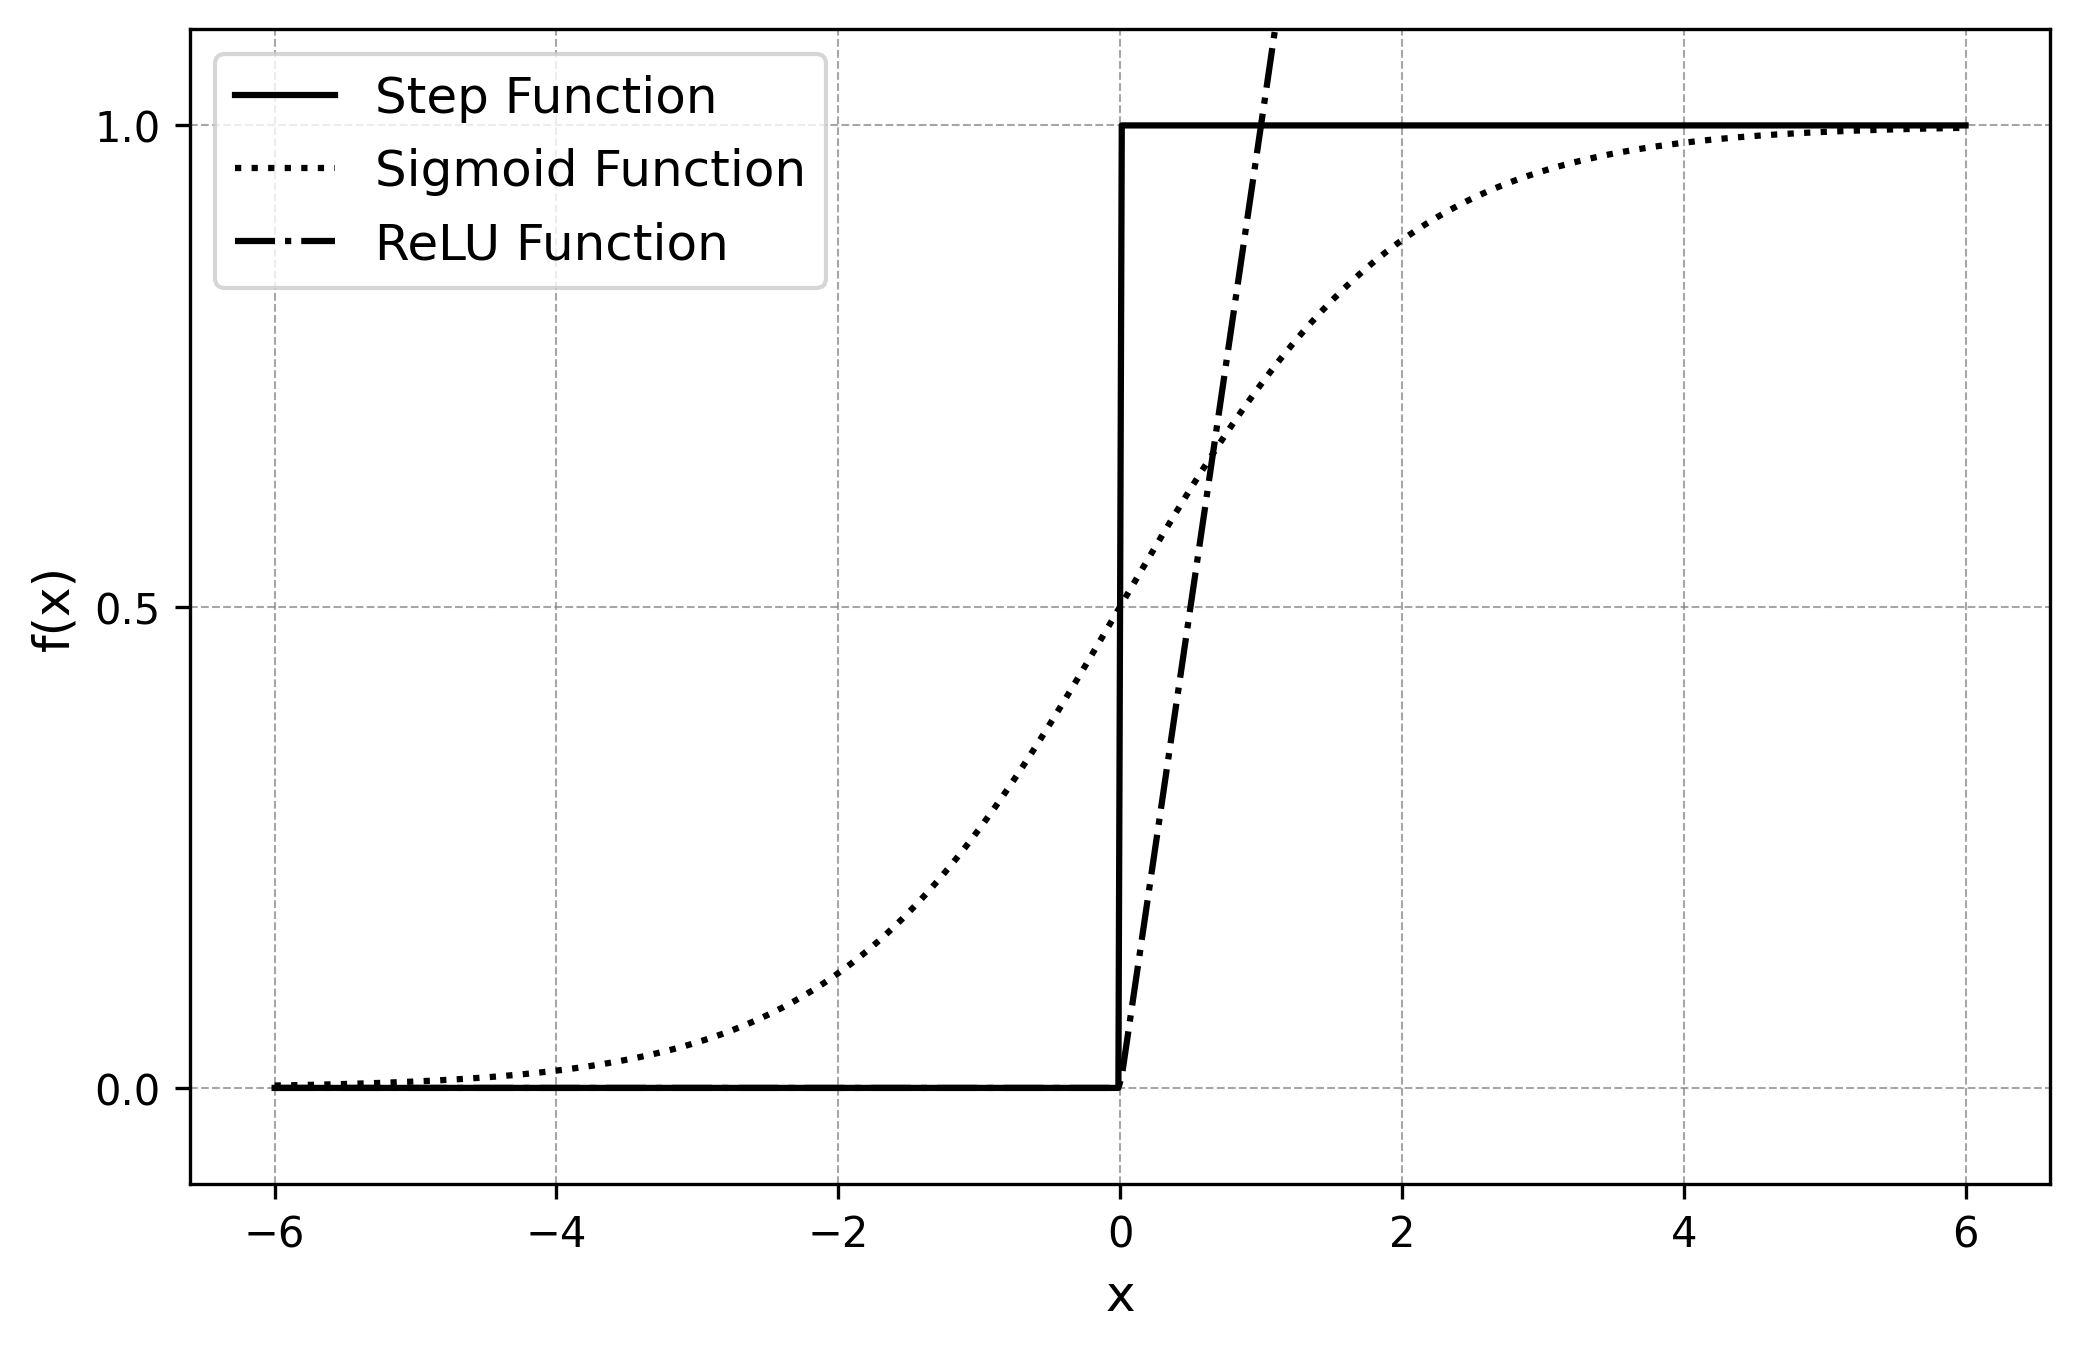
\includegraphics[width=0.9\textwidth]{figures/modelling/activation_functions.png} % file name without extension
	\caption{The Sigmoid Function being a close to the Step Function without being as sensetive to slight changes in $x$ due to its continuity}
	\label{fig:activation_functions}
\end{figure}


With the general structure set up, and assuming that a layout has been chosen for the neural network (e.g. number of layers and number of their coirresponding neurons), the training of the neural network corresponds to adjusting the weights $w$ and the biases $b$ of each neuron in a way, that allows the model to perform the task it is given well. What is means for the model to perform well is defined by a \textit{Loss Function}, that defines a relationship between the output of the model and the correct output (defined by training data) and gives a Loss as output, which is some sort of delta between model prediction and truth. As what it means for a model to perform well heavily depends on the task (regression, binary classification, multiclass classification etc.), but regardless of the task, the goal is always to minimize the Loss Function. A well known Loss Function in regression is the Mean Squared Error (MSE)

\[
\text{MSE} = \frac{1}{n} \sum_{i=1}^{n} (y_i - \hat{y}_i)^2
\]

The training of the Neural Network thus corresponds to adjusting the weights and biases in a way that minimizes the chosen loss function. The algorithm most commonly used for this is called \textit{Backpropagation}.




many Degrees of Freedom, many local maxima


\subsection{Generating Neural Network Model for two Windturbines}

\section{Validation}